% Master thesis template for Ghent University (2021)
%
%
%  !!!!!!!!!!!!!!!!!!!!!!!!!!!!!!!!!!!!!!!!!!!!!!!!!!!!!!!!!!!!
%  !!        MAKE SURE TO SET XeLaTex AS LATEX ENGINE        !!
%  !!!!!!!!!!!!!!!!!!!!!!!!!!!!!!!!!!!!!!!!!!!!!!!!!!!!!!!!!!!!
%  !! For overleaf:                                          !!
%  !!     1. click gear icon in top right                    !!
%  !!     2. select `XeLaTex` in "latex engine"              !!
%  !!     3. click "save project settings"                   !!
%  !!                                                        !!
%  !!!!!!!!!!!!!!!!!!!!!!!!!!!!!!!!!!!!!!!!!!!!!!!!!!!!!!!!!!!!
%
%
%  History
%    2014         Doctoral Thesis of Bruno Volckaert
%    2017         Adapted to master thesis by Jerico Moeyersons
%    2018         Cleanup by Merlijn Sebrechts
%    2021         Update by Marleen Denert and Merlijn Sebrechts with feedback from Leen Pollefliet
%    2022, 2023   Updates by Merlijn Sebrechts
%    2024         Switch to English as first language
%
%  Latest version
%    https://github.com/merlijn-sebrechts/masterproef-template
%

% Note: remove `openany` for printed version
\documentclass[12pt,a4paper,openany,dutch,english]{extbook}
\usepackage[a4paper,includeheadfoot,margin=2.50cm]{geometry}


% By default, LaTeX tries to stretch whitespace between paragraphs on a page in order to reduce whitespace at the end of the page. This sometimes gives ugly results. The following command disables that stretching.
\raggedbottom % Don't reduce whitespace at the end of a page.

\renewcommand{\baselinestretch}{1.2}  % stretch horizontal space between everything by 20%


\usepackage[hyphens]{url} % Break line on hyphens in long urls
\usepackage{graphicx}
\graphicspath{{images/}}
\usepackage{pdfpages}
\usepackage{enumitem}
\usepackage{float}
\usepackage{caption}
\usepackage{subcaption}
\usepackage[toc,page]{appendix}
\usepackage{fontspec}

% Don't indent table of contents, list of figures, and list of tables
\usepackage{tocloft}
\setlength{\cftsecindent}{0pt}    % Remove indent for \section in Table of Contents
\setlength{\cftsubsecindent}{0pt} % Remove indent for \subsection in Table of Contents
\setlength{\cftfigindent}{0pt}    % remove indentation from figures in List of Figures
\setlength{\cfttabindent}{0pt}    % remove indentation from tables in List of Tables

\usepackage{parskip} % Add space between two paragraphs and don't indent the first line of the paragraph

% To generate fake lorem ipsum text
\usepackage{lipsum}



%
% UGent style guide
%
\setmainfont[
	Path=fonts/,
	BoldFont      =UGentPannoText-SemiBold.ttf,
	ItalicFont    =UGentPannoText-Normal.ttf,
	ItalicFeatures={FakeSlant=0.3},
	BoldItalicFont=UGentPannoText-SemiBold.ttf,
    BoldItalicFeatures={FakeSlant=0.3},
]{UGentPannoText-Normal.ttf}
\urlstyle{same} % Also use the default font for URLs


% If you want left justified text, uncomment the line below.
%\usepackage[document]{ragged2e} % Left justify all text

% Style Chapter titles so they have the chapter number in grey.
\usepackage{color}
\definecolor{chaptergrey}{rgb}{0.5,0.5,0.5}
\usepackage[explicit, pagestyles]{titlesec}
\titleformat{\chapter}[display]{\bfseries}{\color{chaptergrey}\fontfamily{lmr}\fontsize{80pt}{100pt}\selectfont\thechapter}{0pt}{\Huge #1}
\titlespacing*{\chapter}{0pt}{-80pt}{30pt}


% Header showing chapter number and title and footer showing page number
\newpagestyle{fancy}{%
  \sethead{} % left
          {} % center
          {\Large\thechapter~~\chaptertitle} %right
  \setfoot{} % left
          {\thepage} % center
          {} %right
  \setheadrule{0pt}
}
\pagestyle{fancy}

% Header showing chapter title and footer showing page number
\newpagestyle{numberless}{%
  \sethead{} % left
          {} % center
          {\Large\chaptertitle} %right
  \setfoot{} % left
          {\thepage} % center
          {} %right
  \setheadrule{0pt}
}

% We use the package `minted` for modern code highlighting.
\usepackage[newfloat,chapter]{minted}
%\SetupFloatingEnvironment{listing}{name=Codefragment, listname=Lijst van codefragmenten} % lang:dutch
\SetupFloatingEnvironment{listing}{name=Code Fragment, listname=List of Code Fragments} % lang:english
\usemintedstyle{pastie} % for other highlighting color schemes, see https://www.overleaf.com/learn/latex/Code_Highlighting_with_minted#Reference_guide

\PassOptionsToPackage{hyphens}{url}
\usepackage{hyperref}
\usepackage{url}

\usepackage[numbers]{natbib}       % For bibliography; use numeric citations
\bibliographystyle{IEEEtran}
\usepackage[nottoc]{tocbibind}     % Put Bibliography in ToC

%
% Defines \checkmark to draw a checkmark
%
\usepackage{tikz}
\def\checkmark{\tikz\fill[scale=0.4](0,.35) -- (.25,0) -- (1,.7) -- (.25,.15) -- cycle;}

%
% For tables
%
\usepackage{booktabs}
\usepackage{array}
\usepackage{ragged2e}  % for '\RaggedRight' macro (allows hyphenation)
\newcolumntype{L}[1]{>{\raggedright\let\newline\\\arraybackslash\hspace{0pt}}m{#1}}
\newcolumntype{C}[1]{>{\centering\let\newline\\\arraybackslash\hspace{0pt}}m{#1}}
\newcolumntype{R}[1]{>{\raggedleft\let\newline\\\arraybackslash\hspace{0pt}}m{#1}}

%
% Support for splitting Dutch words correctly
%
\usepackage{polyglossia}
%\setdefaultlanguage[babelshorthands=true]{dutch} % lang:dutch
\setmainlanguage{english}                       % lang:english

% Manually specify additional hypnations for words
%
% Translated strings. If these aren't set, the English words are used.
%

% \addto\captionsenglish{\renewcommand{\contentsname}{Inhoudsopgave}}   % lang:dutch

% Fix error "Package hyperref Warning: The anchor of a bookmark and its parent's must not be the same. Added a new anchor on ..."
\newcommand{\sectionbreak}{\phantomsection}

% \renewcommand\appendixtocname{Bijlagen}                     % lang:dutch
% \renewcommand\appendixpagename{Bijlagen}                    % lang:dutch


\usepackage[toc,acronym]{glossaries}  % for list of acronyms
\makeglossaries                       % start internal list of acronyms


%
% Set the title and your name
%
%%%%%%%%%%%%%%%%%%%%%%%%%%%%%%%%%%%%%%%%%%%%%%%%%%%%%%%%%%%%%%%%%%%%%%
%
% Add the specific info for your thesis
%
%%%%%%%%%%%%%%%%%%%%%%%%%%%%%%%%%%%%%%%%%%%%%%%%%%%%%%%%%%%%%%%%%%%%%%

\title{Collaborative Compositions: Facilitating Service Orchestration from Cloud to Edge}
\author{Merlijn Sebrechts}







%%%%%%%%%%%%%%%%%%%%%%%%%%%%%%%%%%%%%%%%%%%%%%%%%%%%%
% Add all the acronyms you use in your thesis here. %
% These will be added to the List of Acronyms       %
%%%%%%%%%%%%%%%%%%%%%%%%%%%%%%%%%%%%%%%%%%%%%%%%%%%%%


\newacronym{IP}{IP}{Internet Protocol}
\newacronym{CPU}{CPU}{Central Processing Unit}
\newacronym{vCPU}{vCPU}{Virtual Central Processing Unit}
\newacronym{RAM}{RAM}{Random Access Memory}
\newacronym{TCP}{TCP}{Transmission Control Protocol}
\newacronym{VM}{VM}{Virtual Machine}
\newacronym{IT}{IT}{Information Technology}
\newacronym{API}{API}{Application Programming Interface}
\newacronym{UI}{UI}{User Interface}
\newacronym{GUI}{GUI}{Graphical User Interface}
\newacronym{VPN}{VPN}{Virtual Private Network}
\newacronym{REST}{REST}{Representational State Transfer}
\newacronym{OS}{OS}{Operating System}
\newacronym{HTTP}{HTTP}{HyperText Transfer Protocol}
\newacronym{HTTPS}{HTTPS}{HyperText Transfer Protocol Secure}
\newacronym{SSL}{SSL}{Secure Sockets Layer}
\newacronym{Sysadmins}{sysadmins}{System Administrators}
\newacronym{TOSCA}{TOSCA}{OASIS Topology and Orchestration Specification for Cloud Applications}
\newacronym{ISV}{ISV}{Independent Software Vendors}
\newacronym{M@RT}{M@RT}{Models@run.time}
\newacronym{SA}{SA}{Service Agent}
\newacronym{VNF}{VNF}{Virtual Network Function}
\newacronym{BPMN}{BPMN}{Business Process Modeling Notation}
\newacronym{OA}{OA}{Orchestration Agent}
\newacronym{IoT}{IoT}{Internet of Things}
\newacronym{k8s}{k8s}{Kubernetes}
\newacronym{PaaS}{PaaS}{Platform as a Service}
\newacronym{SSE}{SSE}{Server-Sent Events}
\newacronym{CA}{CA}{Certificate Authority}
\newacronym{CDK}{CDK}{Canonical Distribution of Kubernetes}
\newacronym{DAG}{DAG}{Direct Acyclic Graph}
\newacronym{IQR}{IQR}{Interquartile Range}
\newacronym{QoS}{QoS}{Quality of Service}
\newacronym{Mbps}{Mbps}{Megabits per second}
\newacronym{Km}{Km}{Kilometers}
\newacronym{HnS}{H\&S}{Hub and Spoke}
\newacronym{SLA}{SLA}{Service-Level Agreement}
\newacronym{AWS}{AWS}{Amazon Web Services}
\newacronym{EC2}{EC2}{Elastic Compute Cloud}
\newacronym{FWO}{FWO}{Flemish Fund Scientific Research (Fonds Wetenschappelijk Onderzoek - Vlaanderen)}
\newacronym{VLAIO}{VLAIO}{Flemish Agency for Innovation and Entrepreneurship (Vlaams Agentschap Innoveren en Ondernemen)}
\newacronym{VRT}{VRT}{Flemish Radio and Television (Vlaamse Radio en Televisie)}
\newacronym{SBO}{SBO}{Strategic Basic Research (Strategisch BasisOnderzoek)}
\newacronym{RQ}{RQ}{Research Question}
\newacronym{IEEE}{IEEE}{Institute of Electrical and Electronics Engineers}
\newacronym{SDK}{SDK}{Software Development Kit}
\newacronym{JSON}{JSON}{JavaScript Object Notation}
\newacronym{YAML}{YAML}{Yet Another Markup Language}
\newacronym{ID}{ID}{Identifier}
\newacronym{ISP}{ISP}{Internet Service Provider}
\newacronym{UAV}{UAV}{Unmanned Aerial Vehicle}
\newacronym{STEM}{STEM}{Science, Technology, Engineering and Mathematics}
\newacronym{FSM}{FSM}{Finite State Machine}
\newacronym{ITIL}{ITIL}{Information Technology Infrastructure Library}
\newacronym{CI/CD}{CI/CD}{Continuous Integration and Continuous Deployment}
\newacronym{CD}{CD}{Continuous Deployment}
\newacronym{AIOps}{AIOps}{Artificial Intelligence for IT Operations}



%
%  END OF HEADER
%  The actual latex document content starts here.
%
\begin{document}
\frontmatter
\pagestyle{empty}

% Download the cover sheet from Plato
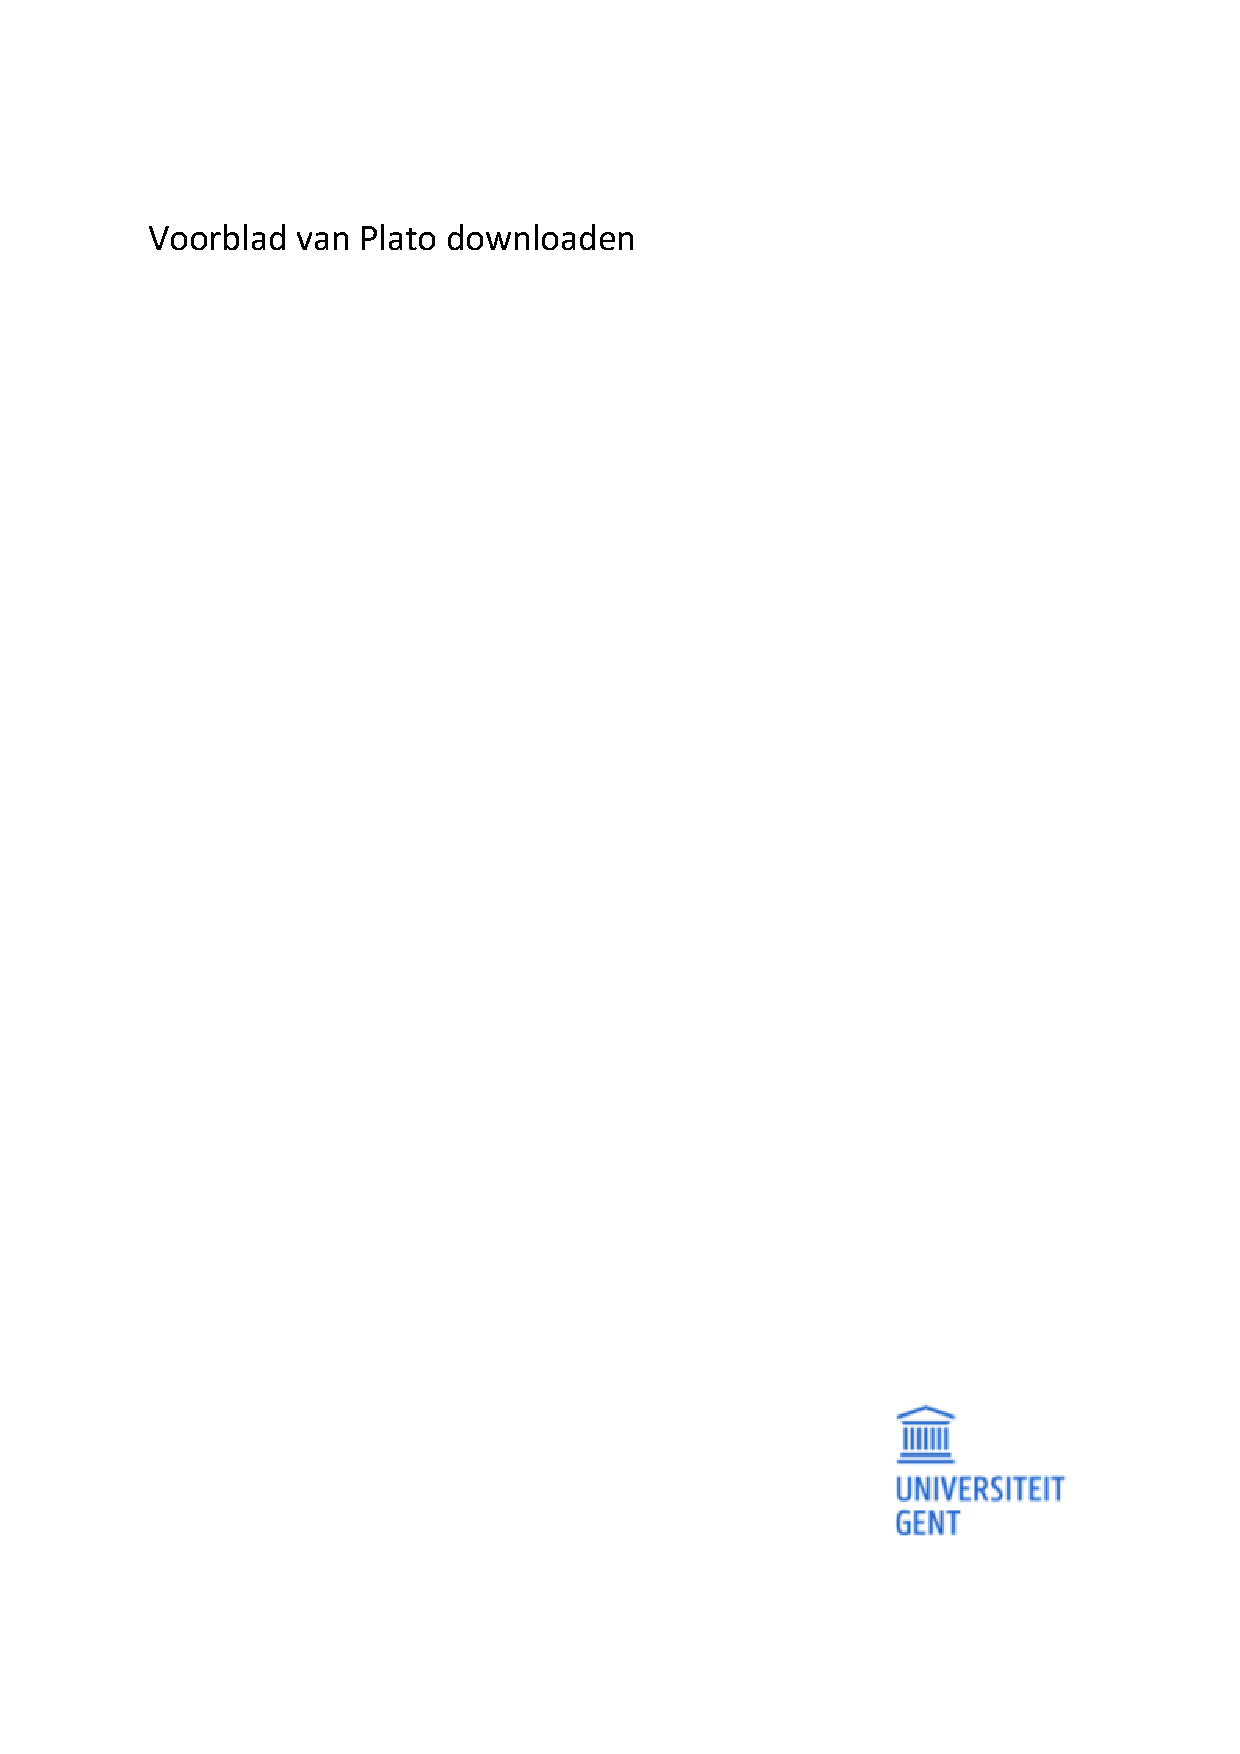
\includepdf{cover-sheet.pdf}

% Only add this Chapter if applicable
\chapter*{Statement of confidentiality}

Confidential up to and including dd/mm/yyyy

Important

This master’s dissertation contains confidential information and/or confidential research results proprietary to Ghent University or third parties. It is strictly forbidden to publish, cite or make public in any way this master’s dissertation or any part thereof without the express written permission of Ghent University. Under no circumstance may this master’s dissertation be communicated to or put at the disposal of third parties. Photocopying or duplicating it in any other way is strictly prohibited. Disregarding the confidential nature of this master’s dissertation may cause irremediable damage to Ghent University. The stipulations mentioned above are in force until the embargo date.

%%%%%%%%%%%%%%%%%%%%%%%%%%%%%%
%    Dutch version           %
%%%%%%%%%%%%%%%%%%%%%%%%%%%%%%
% \chapter*{Melding van vertrouwelijkheid}
%
% Vertrouwelijk tot en met dd/mm/yyyy
%
% Belangrijk
%
% Deze masterproef bevat vertrouwelijke informatie en/of vertrouwelijke onderzoeksresultaten die toebehoren aan de Universiteit Gent of aan derden. Deze masterproef of enig onderdeel ervan mag op geen enkele wijze publiek gemaakt worden zonder de uitdrukkelijke schriftelijke voorafgaande toestemming vanwege de Universiteit Gent. Zo mag de masterproef onder geen voorwaarde door derden worden ingekeken of aan derden worden meegedeeld. Het is verboden om de masterproef te kopiëren of op eender welke manier te dupliceren. Indien de vertrouwelijke aard van de masterproef niet wordt gerespecteerd, kan dit onherstelbare schade veroorzaken aan de Universiteit Gent. Bovenstaande bepalingen zijn van kracht tot en met de embargodatum.
\chapter*{Acknowledgment}

You can use this chapter to give thanks to everyone who has helped bring this thesis to completion.

\chapter*{Explanation regarding the master's thesis and the oral presentation}


This master's dissertation is part of an exam. Any comments formulated by the assessment committee during the oral presentation of the master's dissertation are not included in this text.

%%%%%%%%%%%%%%%%%%%%%%%%%%%%%%
%    Dutch version           %
%%%%%%%%%%%%%%%%%%%%%%%%%%%%%%
%
% \chapter*{Toelichting in verband met het masterproefwerk}
%
% Deze masterproef vormt een onderdeel van een examen. Eventuele opmerkingen die door de beoordelingscommissie tijdens de mondelinge uiteenzetting van de masterproef werden geformuleerd, werden niet verwerkt in deze tekst.
\chapter*{Abstract}
\chaptermark{Abstract}
\addcontentsline{toc}{chapter}{Abstract}  

This chapter should contain three things.

\begin{itemize}
    \item A copy of all the information on the title page of your master's thesis. This includes things like the name of your master's thesis and your advisors.
    \item A one-paragraph description of your master's thesis. This should be 15 to 20 lines long. This should include the context of your master's thesis, the problem statement of your master's thesis. The results of your master's thesis, and the evaluation of the work.
    \item Five keywords that describe the subject best.
\end{itemize}

The chapter should be one page at most.

% How to add the extended abstract:
%
% You should write the extended abstract as a separate overleaf project. Then compile it there, download the PDF, and upload it to this project.
%
% Use the "IEEE conference proceedings template" to create the extended abstract project. 
% https://www.overleaf.com/latex/templates/ieee-conference-template/grfzhhncsfqn
%
% Then download the final PDF, upload it to the root of this project, and point the statement below to the correct file.
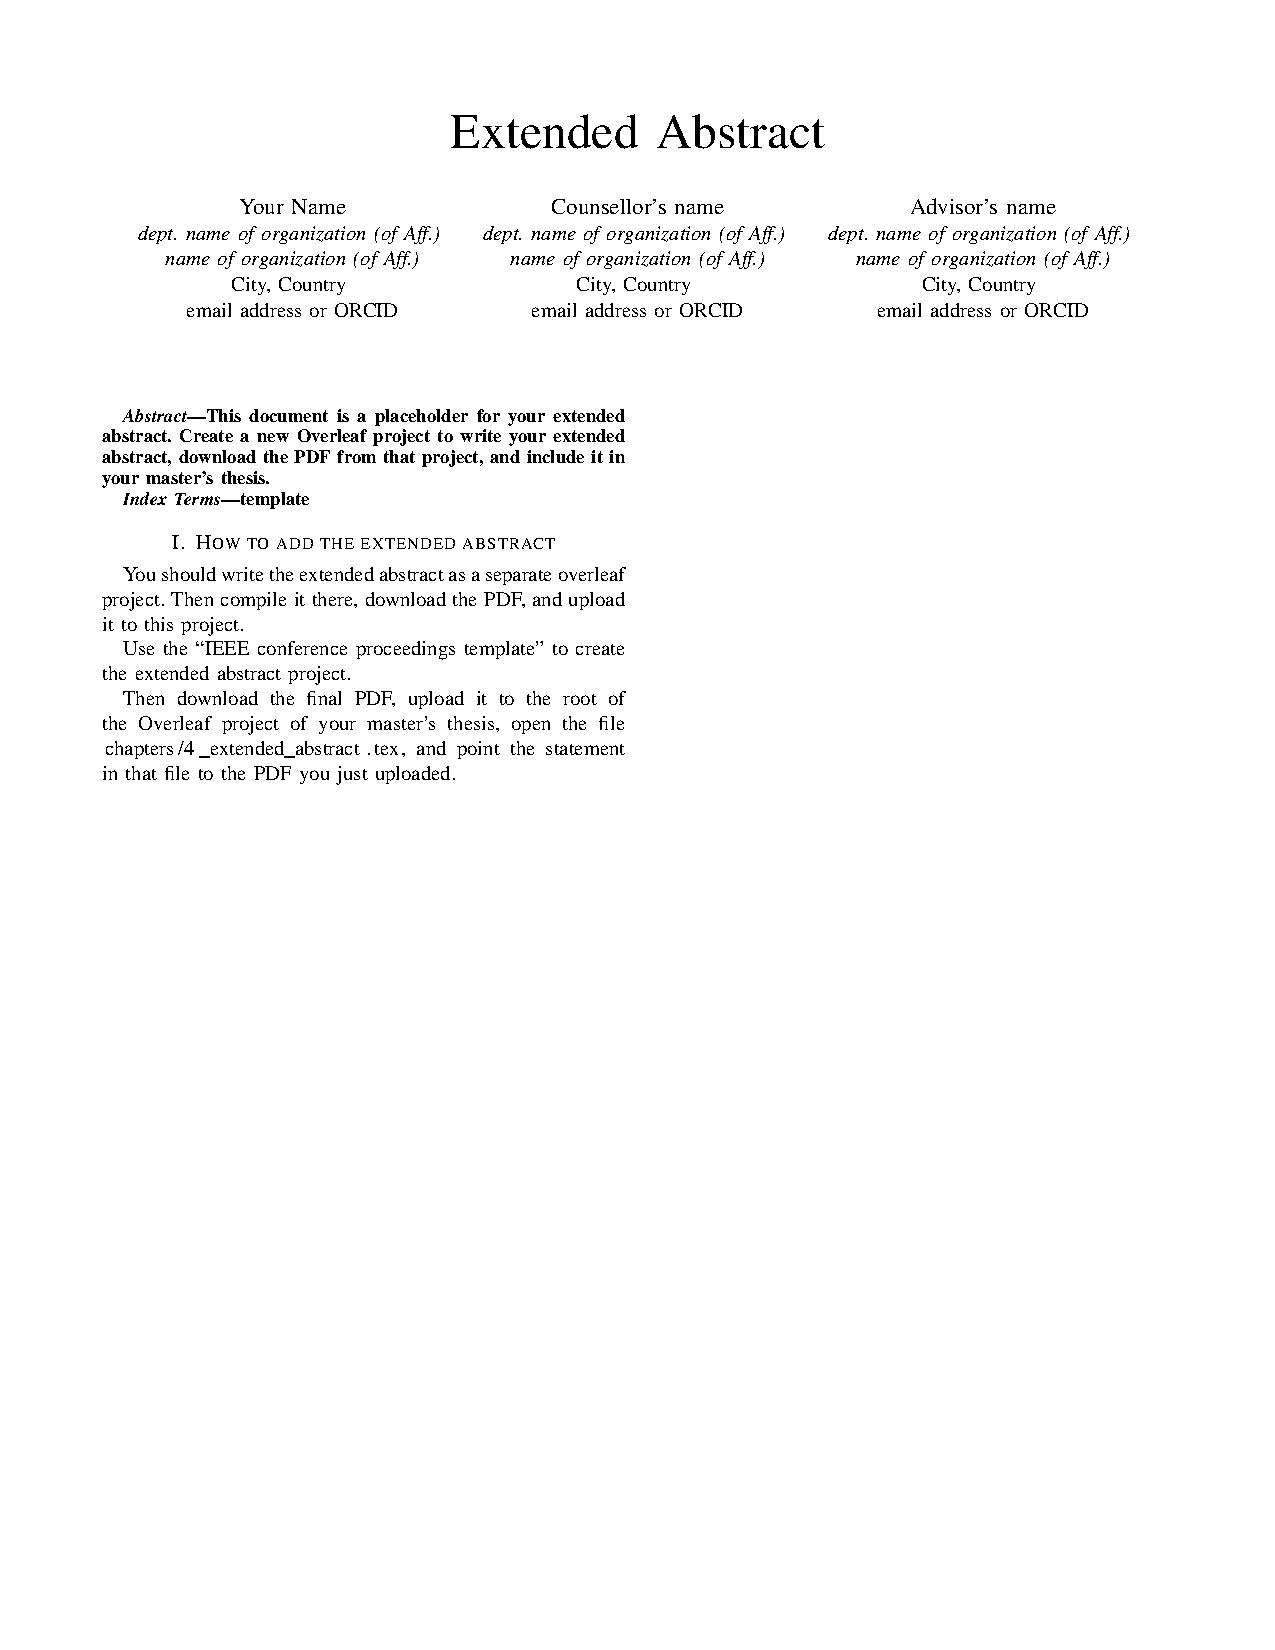
\includepdf[pages={-}]{extended-abstract.pdf}

\tableofcontents\newpage
\listoffigures\newpage
\listoftables\newpage
%%%%%%%%%%%%%%%%%%%%%%%%%%%%%%%%%%%%%%%%%%%%%%%%%%%%%%%%%%%%%%%
%                                                             %
% Note: To add or remove acronyms, modify `personal_data.tex` %
%                                                             %
%%%%%%%%%%%%%%%%%%%%%%%%%%%%%%%%%%%%%%%%%%%%%%%%%%%%%%%%%%%%%%%


% Print the glossary
% \printglossary[type=\acronymtype, title={Lijst van afkortingen}] % lang:dutch
\printglossary[type=\acronymtype, title={List of Acronyms}] % lang:English

\glsaddallunused[\acronymtype]                              % make sure all unused acronyms are in list

\setlist[description]{style=standard} % reset list settings back to default

\listoflistings\newpage

%
% Include the main chapters of the thesis below
% Note: it's best to avoid spaces in filenames as Latex might complain about them.
%
\mainmatter
\pagestyle{fancy} % Use header
\chapter{Introduction}
\label{chap:intro}

\textit{Note: in most master's theses, the Introduction is a full-blow introductory chapter. That's why this chapter is numbered.}

This template supports Unicode natively so special characters like ``é'' and ``ë'' work by default.

As is visible in Figure~\ref{fig:cloud_rollen}, the cloud provider manages the IaaS and PaaS stacks.

\begin{figure}[h]
	\centering
	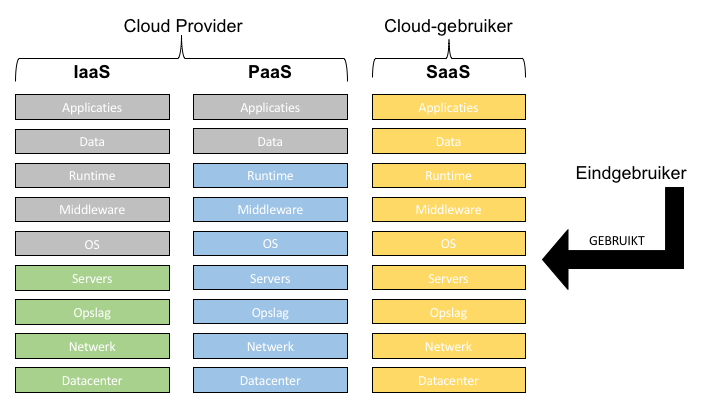
\includegraphics[width=\textwidth]{images/cloud_rollen.png}
	\caption{Image with caption.}
	\label{fig:cloud_rollen}
\end{figure}

Example of a code fragment. Minted supports modern programming languages such as Rust and Golang, and modern configuration formats such as YAML.

\begin{listing}[ht]
\begin{minted}[fontsize=\footnotesize,samepage]{rs}
// This is the main function.
fn main() {
    // Statements here are executed when the compiled binary is called.

    // Print text to the console.
    println!("Hello World!");
}
\end{minted}
\caption{This hello-world code fragment is deceivingly simple. Most rust programs are a lot more difficult to comprehend.}
\end{listing}



\section{Section title}

Table~\ref{tab:resallocschemes} shows an overview of..

\begin{table}[h]
	\centering
	\captionsetup{justification=centering}
	\caption[Overzicht resource-allocatieschema's]{Overzicht resource-allocatieschema's}
	\label{tab:resallocschemes}
	\resizebox{\textwidth}{!}{%
	\begin{tabular}{L{4cm} l C{2cm} c c c c}
		\toprule
		Naam & Jaar & Type  & A | F | P  & Invoer & Uitvoer & Getest  \\ \midrule
		Alicherry et al.~\cite{Alicherry2012} & 2012 & k-sneden & A & G & par\{G\} & S \\
		MCRVMP~\cite{Biran2012} & 2012 & ILP \& GH & A & B\{netwerk\} & VM-plaatsing & C\\
		\bottomrule
	\end{tabular}}
\end{table}

\include{chapters/8_chapter_1.tex}
\chapter{Title of the second chapter}
\label{chap:1}

Text of the second chapter

\section{Section title 1}
\label{sec:1}

Text.

\section{Section title 2}

Text.

\chapter{Title of the third chapter}
\label{chap:2}

Text of the third chapter

\chapter{Title of the fourth chapter}
\label{chap:3}

Text of the fourth chapter

\section{Section title 1}
\label{sec:3}

Text.

\section{Section title 2}

Text.

\chapter*{Conclusion}
\chaptermark{Conclusion}
\addcontentsline{toc}{chapter}{Conclusion}  

Fill in..

\chapter*{Future Work}
\chaptermark{Future Work}
\addcontentsline{toc}{chapter}{Future Work}  

This chapter explains what the next steps are to continue the research and innovation of your master's thesis. Are there any additional features of research directions that are interesting? Are there ways in which your solution can be improved?

\chapter*{Sustainability reflection}
\chaptermark{Sustainability reflection}
\addcontentsline{toc}{chapter}{Sustainability reflection}  

This chapter is only for the engineering technology ("industrieel ingenieur") students. It contains a sustainability reflection. You can intepret sustainability very broadly. For example, this chapter can include one or more of the following.

\begin{itemize}
    \item Placing the work in a broader societal context. For example, how does this work impact or contribute to recent societal change such as digital transformation or the AI revolution?
    \item Explaining how the work contributes to the implementation of the United Nations (UN) Sustainable Development Goals (SDGs). For more information, see \url{https://en.wikipedia.org/wiki/Sustainable_Development_Goals} and \url{https://www.sdgs.be/nl/sdgs}.
    \item Reflecting on the ethical impact of this thesis or the used datasets. For example, how does this impact people's privacy? Is there bias available in the datasets? Could this be used for military or dual-use purposes?
    \item Investigating how the resulting work conforms to relevant laws or technical standards such as the GDPR, AI act and the CRA.
\end{itemize}

\renewcommand\bibname{References}
\bibliography{references.bib}

%%%%%%%%%%%%%%%%%%%%%%%%%%%%%%
%    Dutch version           %
%%%%%%%%%%%%%%%%%%%%%%%%%%%%%%
% \renewcommand\bibname{Referenties}
% \bibliography{references.bib}

\begin{appendices}
\section*{Attachment A}
\addcontentsline{toc}{section}{Attachment A}  

Attachment description.



\newpage
\section*{Attachment B}
\addcontentsline{toc}{section}{Attachment B}  

Attachment description.

\end{appendices}

%%%%%%%%%%%%%%%%%%%%%%%%%%%%%%
%    Dutch version           %
%%%%%%%%%%%%%%%%%%%%%%%%%%%%%%
% \begin{appendices}
% \section*{Bijlage A}
% \addcontentsline{toc}{section}{Bijlage A}  

% Toelichting bijlage.



% \newpage
% \section*{Bijlage B}
% \addcontentsline{toc}{section}{Bijlage B}  

% Toelichting bijlage.

% \end{appendices}


\pagestyle{numberless} 
\pagestyle{empty}
\include{chapters/12_appendices.tex}

\end{document}
